\chapter{Evaluation}
\label{ch:Evaluation}

This chapter provides information about the input data acquired from different sources, the implementation, the results of the electricity forecasts, how they were obtained and an evaluation considering the performance and the quality of the output.\\
%In this chapter, the used methods will be evaluated and critically regarded considering their performance and the quality of their outputs.\\


\section{Data}
\label{sec:data}

In this section, the different types of data that are used within this thesis are presented. After that, the process of data preprocessing is briefly examined.\\

%Of course choosing data sources as well as sorting and cleaning the data also requires a certain amount of time and effort. Thus it will be explained hereinafter how this has been done for the data used in this thesis.


\subsection*{ECMWF}

The data used in this thesis originates from \gls{ecmwf}, which is a research institute that produces global numerical weather predictions and other data. It is time series based and for each timestamp there is a 2-dimensional array referred to by longitude and latitude respectively.\\

It must be mentioned, that, as the data that is used, has been reanalysed. This means, that the expected error is likely to be smaller than if working with real-time data.\\

As data parameters, there are also longitude and latitude, where the longitude is chosen to be from 5.5 to 15.5 and the latitude from 47 to 55.5. As the resolution of the used grid is at 0.25 degrees, this results in a total of 1435 grid points per timestamp. As the range of the data from \gls{ecmwf} extends from 2015/1/1 to 2018/12/31, there is a total of 1461 days with each 24 timestamps due to the 1 hours frequency and thus 35064 timestamps. Considering that there is a value for each point in the grid and every timestamp, there are 50316840 values for each variable and thus 654118920 values for 13 variables.\\

%In \Cref{fig:maxvar4_maps}, there are maps of Germany plotted, showing the 2 metre temperature at the four times with the highest variance.
%\Cref{fig:maxvar4_maps} shows four plots of the data on a map of Germany and \Cref{fig:isin_compare}. In this case the temperature measured at 2 metres is visualized.\\

%\begin{figure}[h!]%
%\centering
%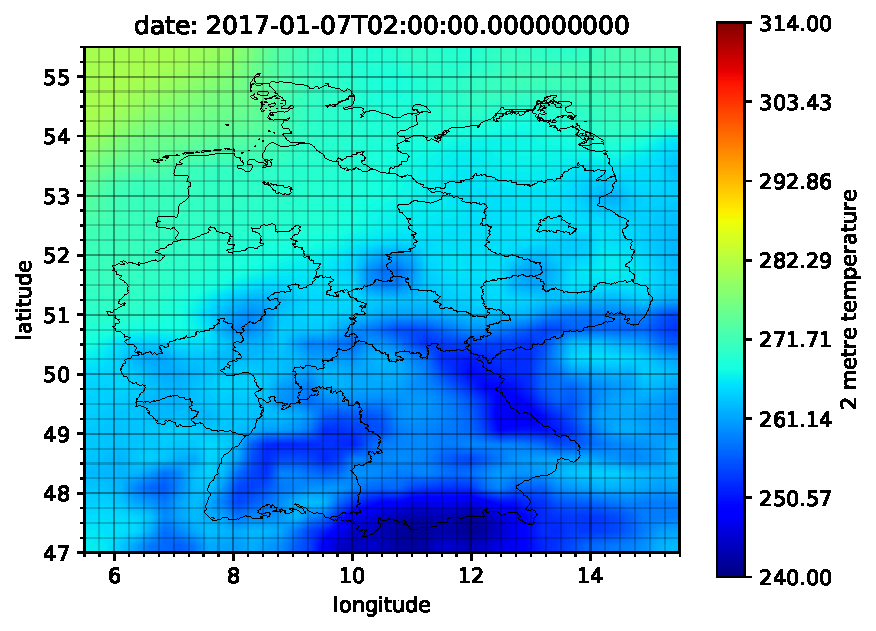
\includegraphics[width=\textwidth]{plots/0_2017010702_20190617161317}%
%\caption{Map showing day with lowest temperature in germany.}%
%\label{fig:0_2017010702_20190617161317}%
%\end{figure}

\begin{figure}[h!]%
\centering
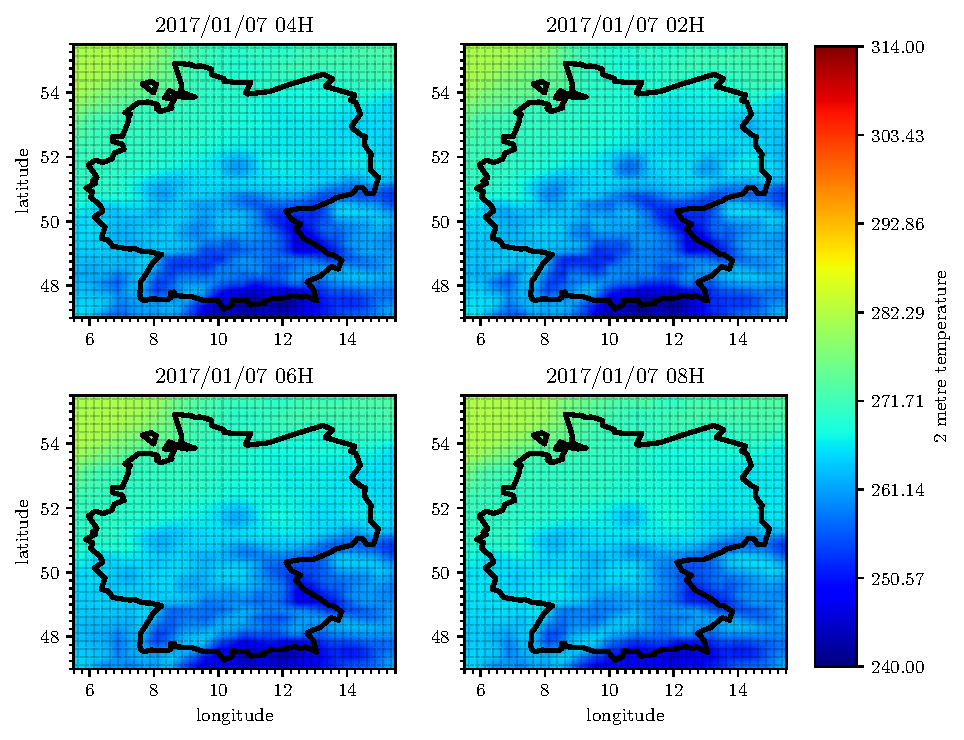
\includegraphics[width=\textwidth]{plots/t2m/bundles/maxvar4_maps}%
\caption{Four maps showing the four times with the highest 2 metre temperature variance in Germany, where top left is the highest, top right the second highest, bottom left the third highest and bottom right the fourth highest variance.}%
\label{fig:maxvar4_maps}%
\end{figure}

In order to reduce complexity, a shapefile of the \acrshort{nuts} dataset was used. The shapefile contains all countries in the EU. The shape of Germany was filtered from this data and each point in the dataset is checked whether it is within Germany or not. The result can be seen in the left figure in \Cref{fig:isin_compare}. An example for a complete map without filtering is shown in \Cref{fig:maxvar4_maps}, where a map of the four times with the highest variance in 2 metre temperature are displayed, respectively. The filtered map first is stored in a numpy.ndarray and then applied on the data to mask unwanted data. The filtered map is visualized in the right figure in \Cref{fig:isin_compare}. The same process was made for NUTS 3 level districts which later in this section considering population data.\\

\begin{figure}[h!]%
	\centering
	\begin{subfigure}{.5\textwidth}
		\centering
		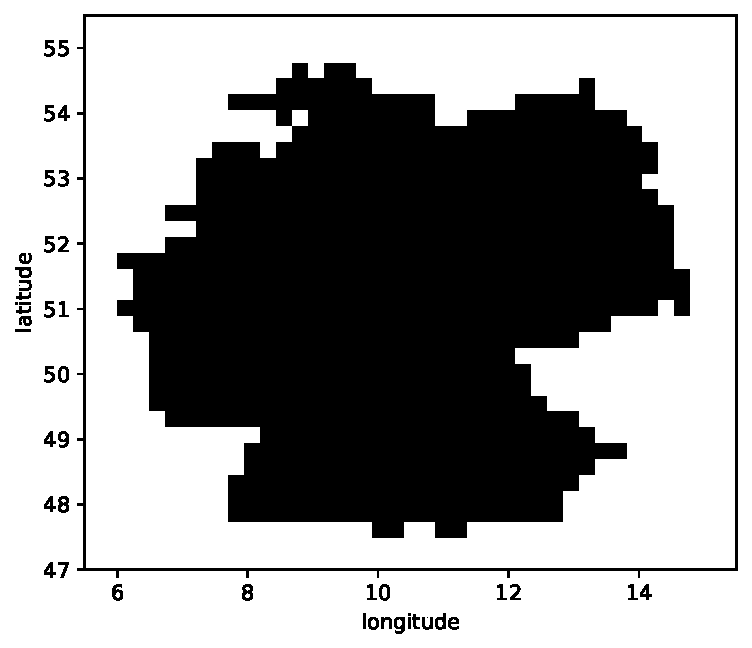
\includegraphics[width=.85\textwidth]{plots/isinDE}%
		\label{fig:isinDE}%
	\end{subfigure}%
	\begin{subfigure}{.5\textwidth}
		\centering
		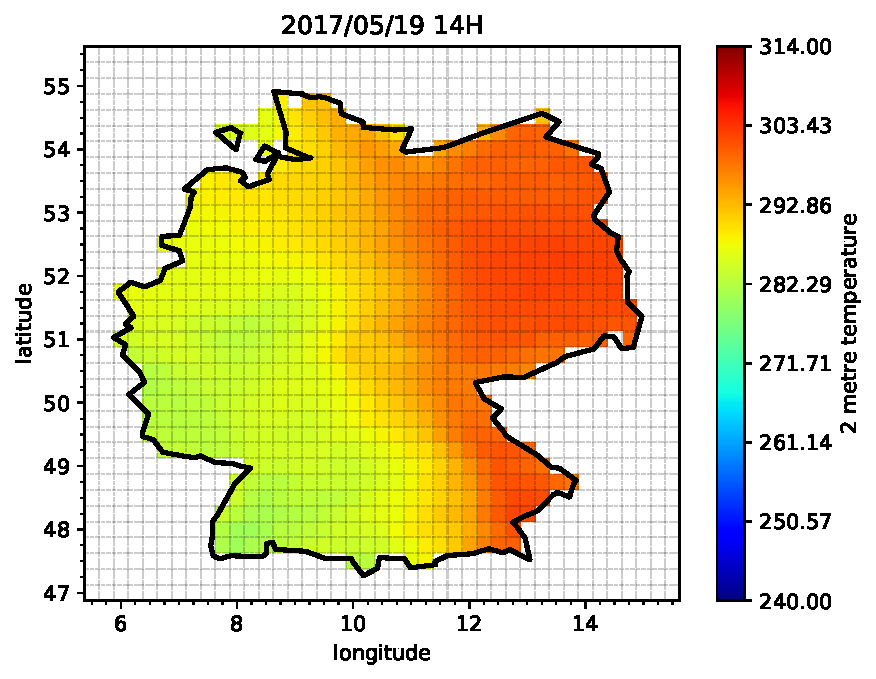
\includegraphics[width=.95\textwidth]{plots/t2m/maxvar/0_map_isin}%
		\label{fig:t2m_maxvar_0_map_isin}%
	\end{subfigure}
	\caption[2D boolean numpy.ndarray (left) used to filter grid squares within Germany. It was created by using a shapefile of Germany from Eurostat and checking for each point of the grid if it is within the shapefile. When applied to the weather data, only relevant data within Germany is obtained (right).]{2D boolean numpy.ndarray (left) used to filter grid squares that are within Germany. It was created by using a shapefile of Germany from Eurostat\footnotemark and checking for each point of the grid whether it is within the shape. When applied to the weather data, only relevant data within Germany is obtained (right).}
	\label{fig:isin_compare}
\end{figure}
\footnotetext{\url{https://ec.europa.eu/eurostat/de/web/gisco/geodata/reference-data/administrative-units-statistical-units/nuts}}

The initial dataset contains a set of variables listed in \Cref{tab:wvars} where also the units, mean, min and max are shown for each variable respectively.\\

\begin{table}[h!]%
\rowcolors{2}{white}{gray!25}
\centering
\caption[Exogenous weather variables used to forecast the load including min, max values from \acrshort{ecmwf}.]{List of exogenous weather variables used to forecast the load including min, max values from \acrshort{ecmwf}\footnotemark.}
\footnotesize
\begin{tabularx}{\linewidth}{Llrrr}
\tablehead variable name & \tablehead units & \tablehead mean & \tablehead min & \tablehead max \\\hline
10 metre U wind component & $m~s^{-1}$ & 1.05 & -18.80 & 22.91\\
10 metre V wind component & $m~s^{-1}$ & 0.57 & -21.51 & 20.00\\
2 metre temperature & $K$ & 282.97 & 240.97 & 313.26\\
Leaf area index, high vegetation & $m^{2}~m^{-2}$ & 1.84 & -0.00 & 4.90\\
Leaf area index, low vegetation & $m^{2}~m^{-2}$ & 2.24 & -0.00 & 3.84\\
Low cloud cover & $(0~-~1)$ & 0.38 & 0.00 & 1.00\\
Soil temperature level 1 & $K$ & 283.12 & 257.68 & 313.64\\
Surface latent heat flux & $J~m^{-2}$ & -166716.23 & -2203977.00 & 359411.00\\
Surface net thermal radiation & $J~m^{-2}$ & -192527.73 & -664669.00 & 142945.02\\
Surface sensible heat flux & $J~m^{-2}$ & -41139.49 & -1730277.12 & 826042.00\\
Total cloud cover & $(0~-~1)$ & 0.66 & 0.00 & 1.00\\
Total column rain water & $kg~m^{-2}$ & 0.01 & -0.00 & 2.73\\
Total sky direct solar radiation at surface & $J~m^{-2}$ & 282134.31 & -0.12 & 3088320.00\\
\end{tabularx}
\label{tab:wvars}
\end{table}
\footnotetext{\url{https://www.ecmwf.int/en/forecasts/datasets/browse-reanalysis-datasets}}


\subsection*{Load Data}

Besides weather data used to refine the forecasting results, also historic load data was needed. Therefore data has been retained from Open Power System Data\footnote{\url{https://data.open-power-system-data.org/time_series/}}. \Cref{fig:t2m_mean_18A5_twofold_24F} shows the distribution of loads over time with one point per day at 12 am UTC time. The color shows the mean temperature measured at 2 metres. The same data in a single plot is added in the Appendix as \Cref{fig:t2m_mean_2015010112_2018123112_24F}, it is split here in two plots for better distinction of single points.\\

%\begin{figure}[h!]%
%\centering
%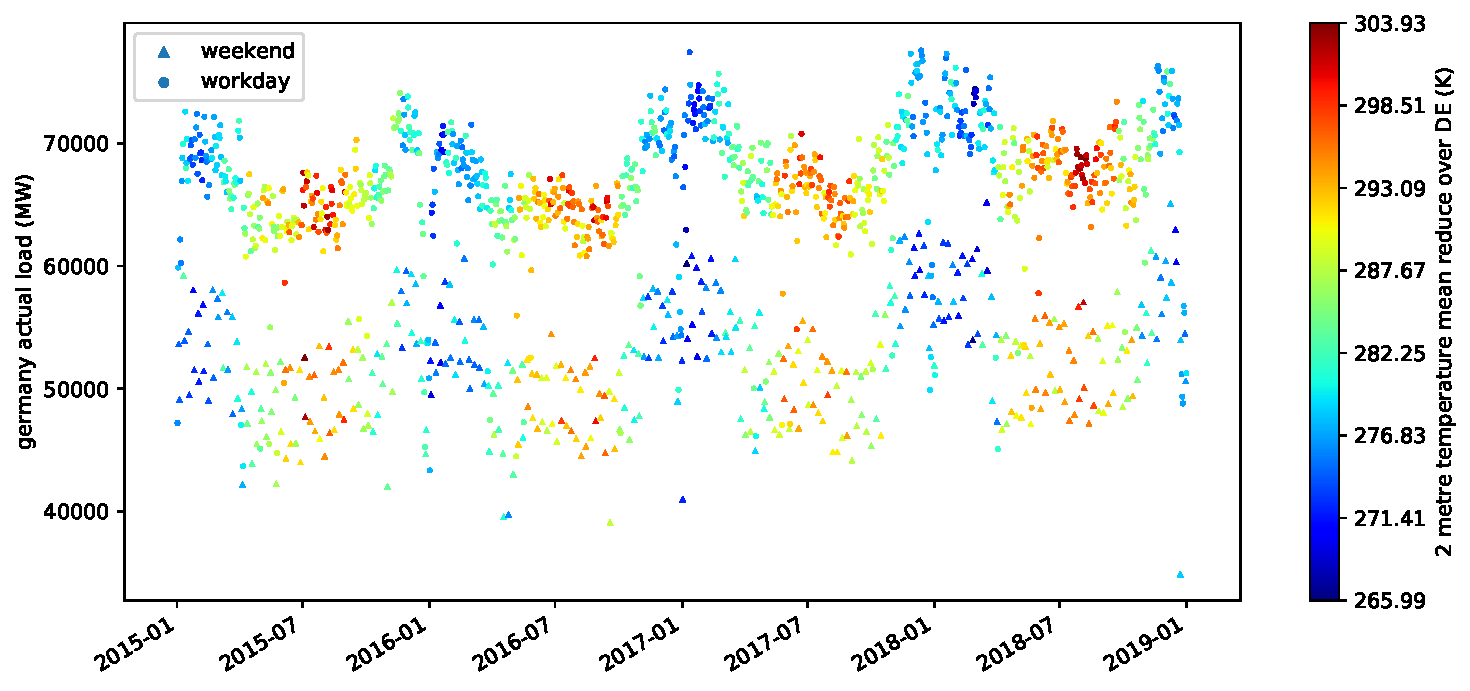
\includegraphics[width=\textheight,angle=-90,origin=c]{plots/t2m_mean_2015010112_2018123112_24F}%
%\caption{Load curve with mean of 2 metre height measured temperature in germany as color from 2015/1/1 to 2018/12/31 with one single point per day at 12am utc time respectively.}%
%\label{fig:t2m_mean_2015010112_2018123112_24F}%
%\end{figure}

\begin{figure}[H]%
	\centering
	\begin{subfigure}{.5\textwidth}
		\centering
		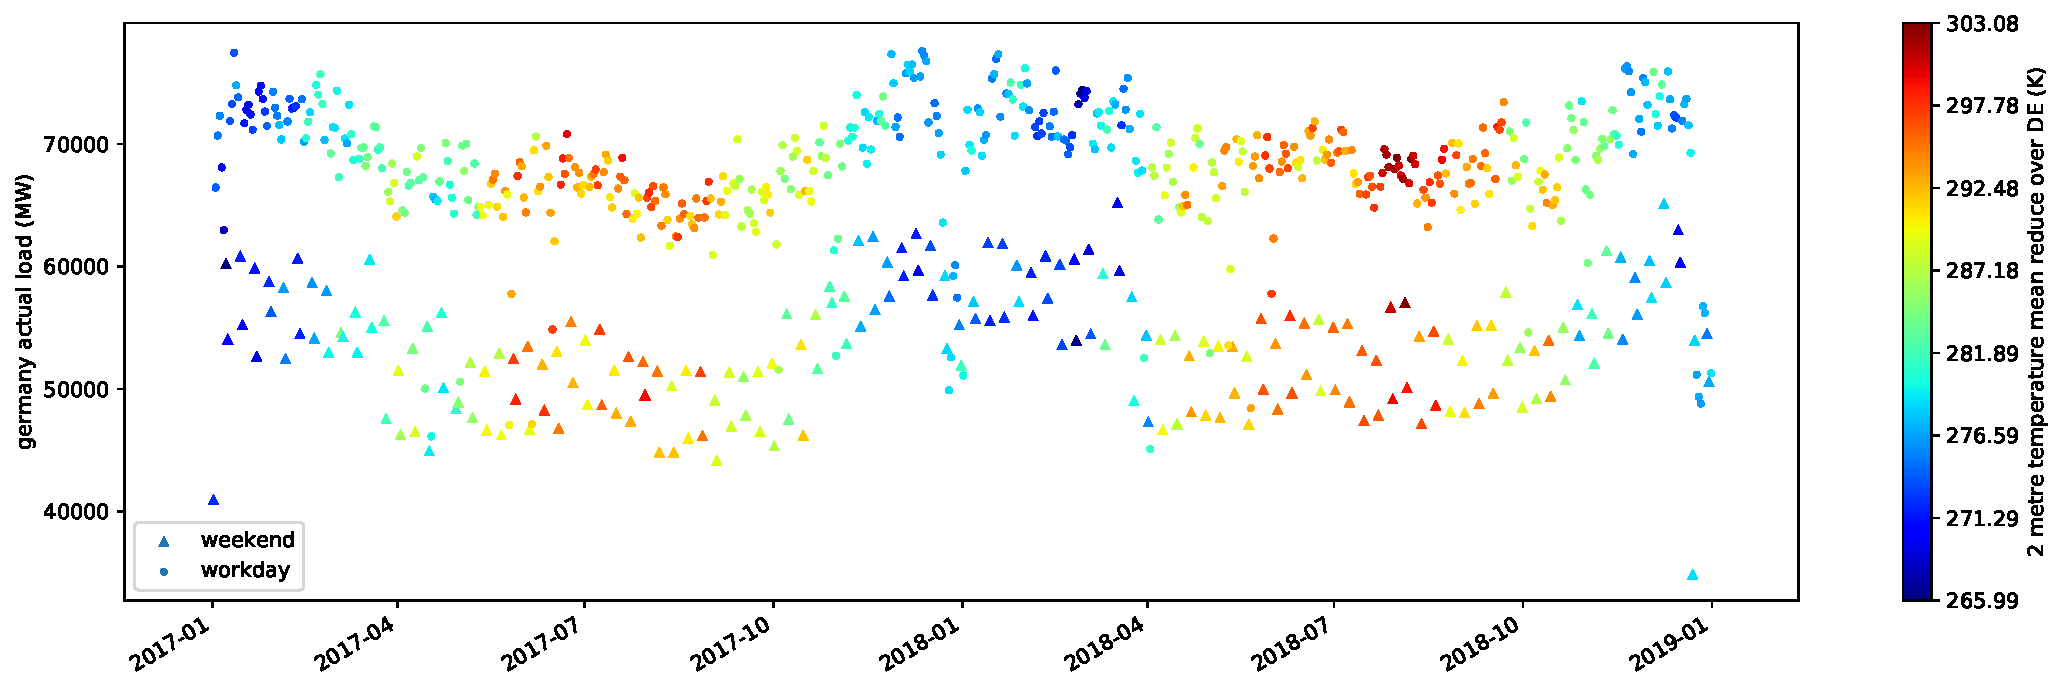
\includegraphics[width=2.9\textwidth,angle=-90,origin=c]{plots/plot_load_time_func/t2m_mean_18A5_2017010112_2018123112_24F}%
		\label{fig:t2m_mean_18A5_2017010112_2018123112_24F}%
	\end{subfigure}%
	\begin{subfigure}{.5\textwidth}
		\centering
		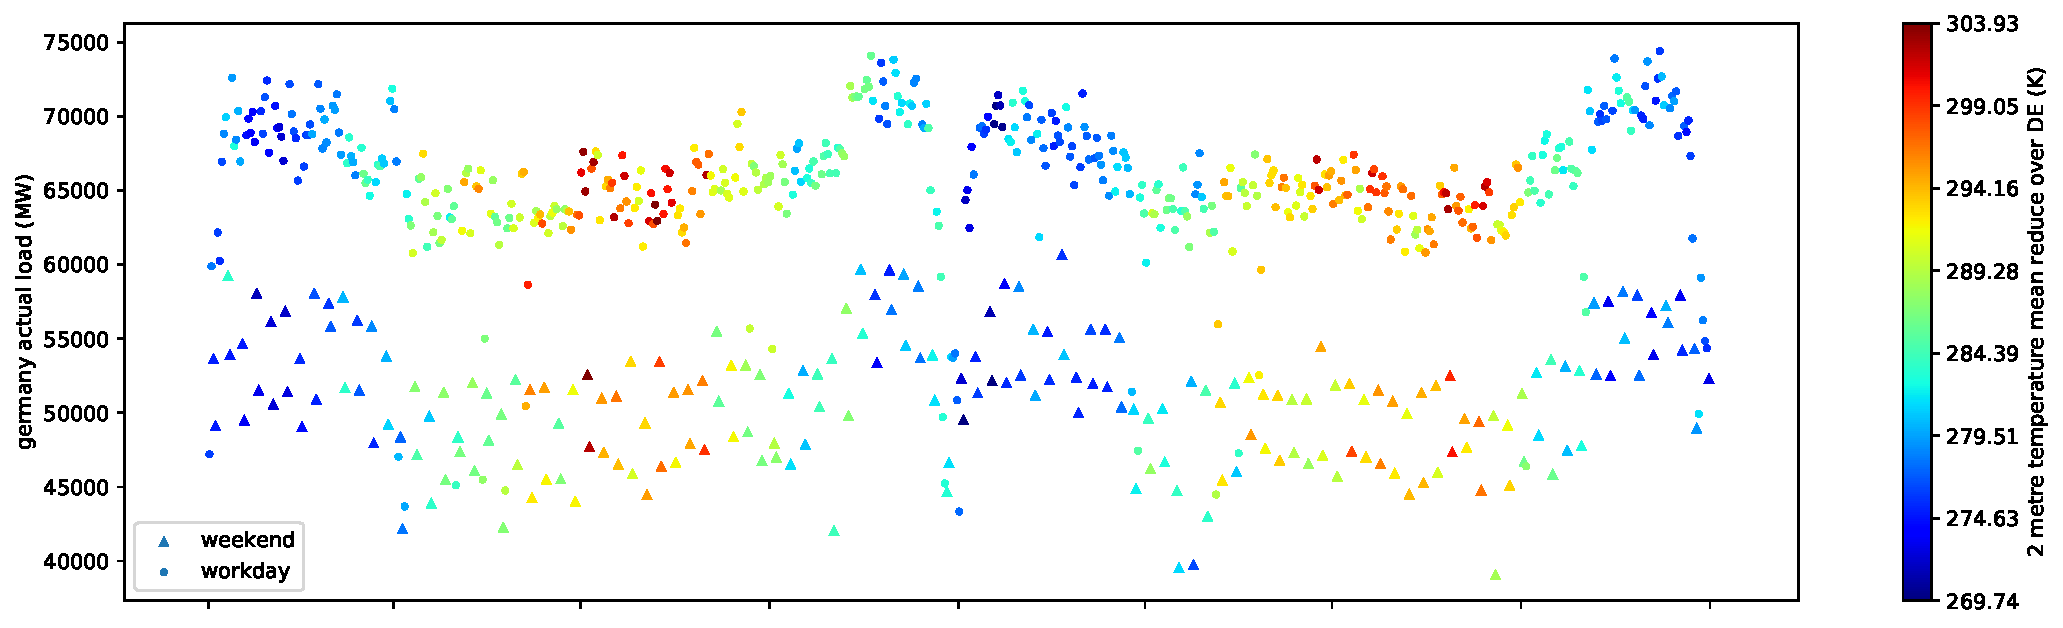
\includegraphics[width=2.9\textwidth,angle=-90,origin=c]{plots/plot_load_time_func/t2m_mean_18A5_2015010112_2016123112_24F}%
		\label{fig:t2m_mean_18A5_2015010112_2016123112_24F}%
	\end{subfigure}
	\caption{Load curve with mean of 2 metre measured temperature in Germany as color from 2015/1/1 to 2018/12/31 with one single point per day at 12 AM UTC time respectively.}
	\label{fig:t2m_mean_18A5_twofold_24F}
\end{figure}


\subsection*{Population Data}

For further improvement and in order to filter important points in the grid, population data for Germany has been acquired from Eurostat\footnote{\url{https://ec.europa.eu/eurostat/data/database}}. The data is being visualized in \Cref{fig:demo2018_logscale} with a logarithmic scale to improve visual distinction between the different regions which would be difficult for a non-logarithmic scale.\\

\begin{figure}[h!]%
\centering
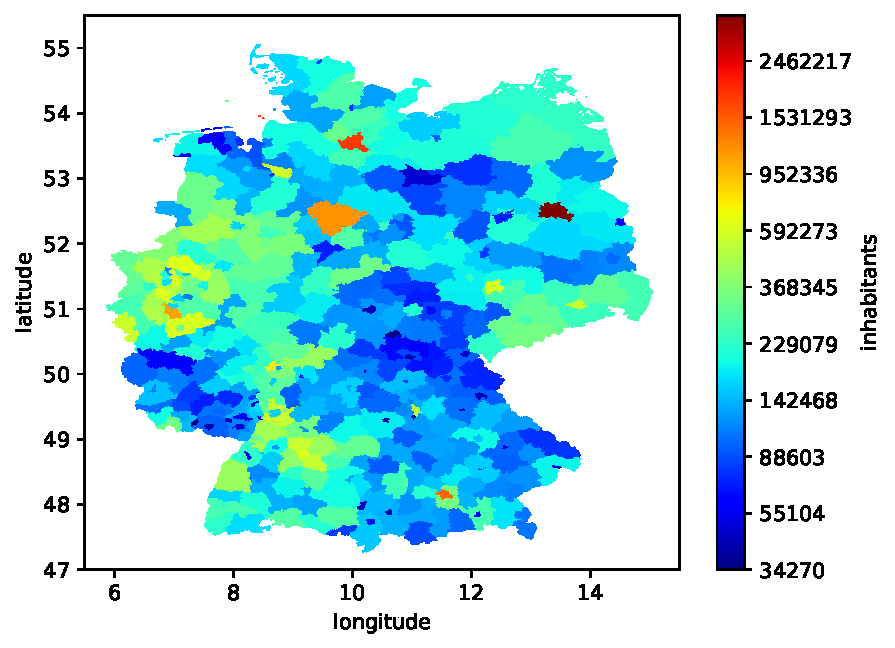
\includegraphics[width=\textwidth]{plots/demo/demo2018_logscale}%
\caption{Population of Germany for each region respectively using a logarithmic scale for better distinction.}%
\label{fig:demo2018_logscale}%
\end{figure}


\subsection*{Data Preprocessing}

As both, the load data and the weather data come from trustful sources, the need for data preprocessing is very limited. Nevertheless, there is still some missing or doubtful data. \Eg the values for the first months of the load data, that are located at the end of 2014, are much smaller than those after 2015. There is a possibility that this might be correct data, but to avoid uncertainties, only data from the beginning of 2015 to the end of 2018 is used. Also, there are some missing values that are linearly interpolated over time. The same about missing values applies to the weather data. Here it would also be possible to interpolate over locality, but for some time steps, there are no values at all, which is why temporal interpolation makes more sense in this case.\\


\section{Implementation}
\label{sec:prog}

This section will first outline which programming language is used and why. After that there are two points about the documentation and an additional comment about the process of implementation.\\

For the programming part, Python\footnote{\url{https://www.python.org/}} 3.6+ has been chosen, as there is a variety of libraries to process all used file formats and because it tends to be a time saving language, also for visualization. Furthermore, Python has a highly vibrant and supportive community.\\

In regard to coding styles, especially when it comes to docstrings, the numpy conventions are used. This style is based on the reStructuredText\footnote{\url{http://docutils.sourceforge.net/rst.html}} markup syntax. The three major points for this are first, that it is a popular and often used style, second, it is also a visually oriented style which means, that it is easy to read as can be seen in \Cref{fig:wing_docstrings} and last, it is supported by several automated documentation tools that create a PDF or HTML based documentation from existing source code with docstrings. For this purpose, the Sphinx\footnote{\url{http://www.sphinx-doc.org}} tool is used.\\

\begin{figure}[h!]%
\centering
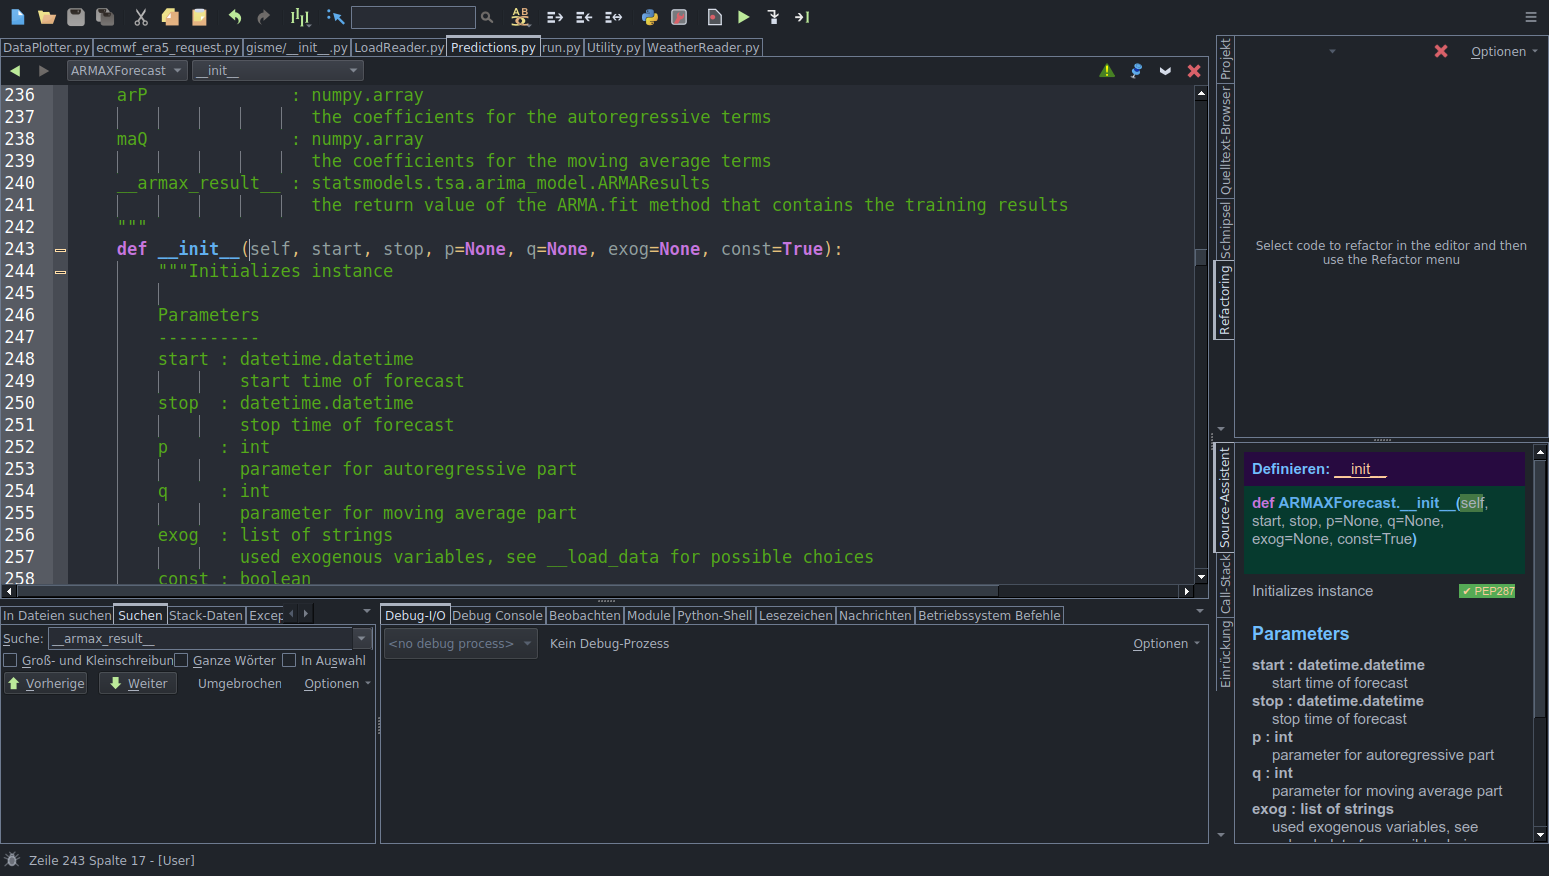
\includegraphics[width=\textwidth]{logos/Predictions_Wing_001}%
\caption[Python code and numpy docstring in the Wing IDE.]{Python code and numpy docstring in the Wing IDE.\footnotemark.}%
\label{fig:wing_docstrings}%
\end{figure}
\footnotetext{\url{https://wingware.com/}}

Considering the \gls{arma} model, the statsmodels\footnote{\url{http://www.statsmodels.org/stable/index.html}} package is used. During the process of implementation, it turned out that the forecasting functionality of this model does not behave correctly when using exogenous data. Therefore, this had to be implemented newly. At this point, I would like to thank Kaleb Phipps\footnote{\url{https://www.iai.kit.edu/2154_2880.php}} who provided some very useful code, saving me a lot of time that would have otherwise been spent for debugging.\\


\section{Results}
\label{sec:results}

In this section, there are first two points about model selection. After that, the acquired results are presented.\\

%At this point, I would like to thank Kaleb Phipps\footnote{\url{https://www.iai.kit.edu/2154_2880.php}} who provided some very useful code, saving me a lot of time that would have otherwise been spent for debugging due to indexing issues. Also, I would like to thank Nicole Ludwig again\footnote{\Cref{ack:nicole}}, since she put a lot of effort in bug tracing.\\ % TODO put this in acknowledgements

\subsection*{Model Selection}

The first steps for estimating reasonable values for $p$ and $q$ values of an \gls{arma} often are the \gls{acf} and the \gls{pacf}. The respective plots in \Cref{fig:acf_compare} may suggest a $p$ value between 3 and 6 and a $q$ value between 2 and 4.\\

\begin{figure}[h!]%
	\centering
	\begin{subfigure}{.5\textwidth}
		\centering
		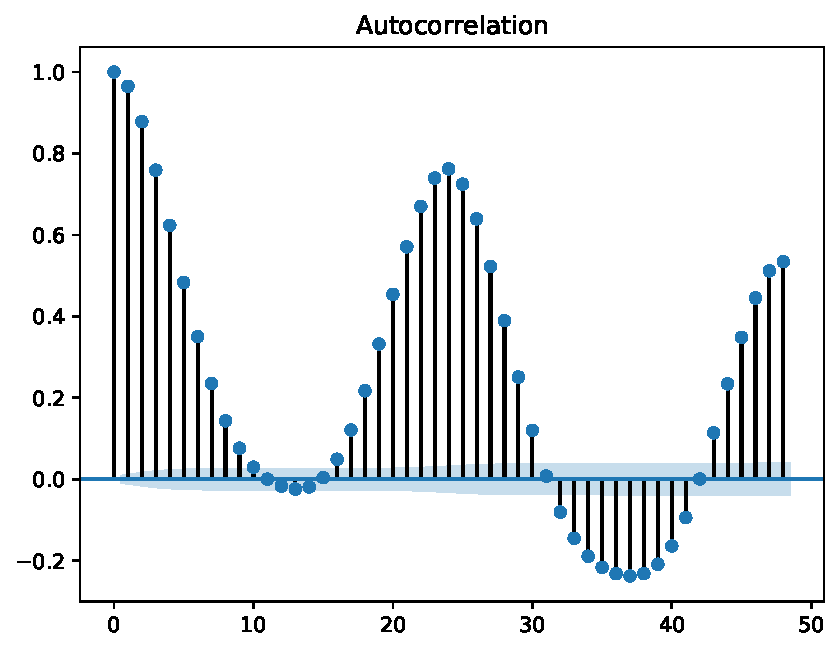
\includegraphics[width=\textwidth]{plots/ACF/load_48lags_ndiff0_hstep1}%
		\caption{}
		\label{fig:acf_load_lags48}%
	\end{subfigure}%
	\begin{subfigure}{.5\textwidth}
		\centering
		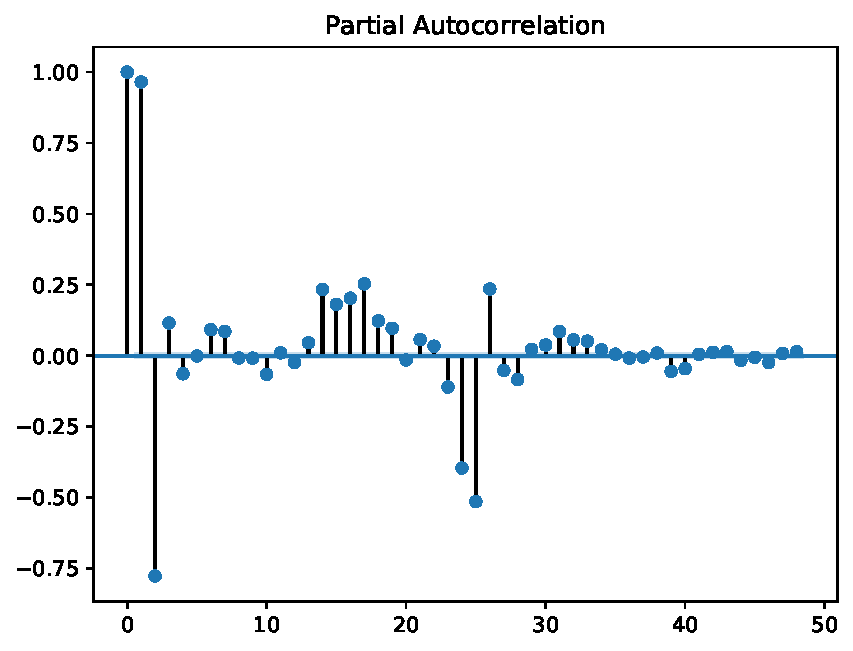
\includegraphics[width=\textwidth]{plots/PACF/load_48lags_ndiff0_hstep1}%
		\caption{}
		\label{fig:pacf_load_lags48}%
	\end{subfigure}
	\caption{Autocorrelation (a) and Partial Autocorrelation (b) plots used to select the order of \acrshort{arma} and \acrshort{armax} models.}
	\label{fig:acf_compare}
\end{figure}

Information criteria are often used metrics for \gls{arma} models when $p$ and $q$ are limited to a small range of numbers. Then all those models are fitted and the respective information criteria are computed. In general, as can be seen in \Cref{tab:ic_table}, the \gls{aic}, \gls{bic} and \gls{hqic} get smaller for higher $p$ and $q$ values, which is the desired behaviour, as smaller values are better when comparing information criteria for different models that use the same data. However, for higher $p$ and $q$ values of 4 or 5, it can be observed, that the information criteria do not decrease considerably. Thus, it can be said, that appropriate $p$ and $q$ values may be found between 2 and 4. The missing values in the table result from cases where some parameters could not be computed.\\

\begin{table}
\rowcolors{2}{white}{gray!25}
\centering
\caption{Information Criteria for \acrshort{arma} models without exogenous inputs using training data from 2015/01/01 to 2017/12/31 to compare for model selection with number of \acrshort{ar} terms on one axis and number of \acrshort{ma} terms on the other.}
\footnotesize
\begin{tabularx}{\linewidth}{p{.6cm}p{1.2cm}XXXXXX}
& \tablehead MA(q) >\newline AR(p) v & 0 & 1 & 2 & 3 & 4 & 5\\\hline
AIC\newline ~BIC\newline \rule{0pt}{1em}HQIC & 1 & 489489.23\newline 489513.76\newline 489497.15 & 472851.05\newline 472883.76\newline 472861.61 & 467543.07\newline 467583.96\newline 467556.27 & 466091.08\newline 466140.14\newline 466106.92 & 465622.11\newline 465679.35\newline 465640.59 & 464728.34\newline 464793.76\newline 464749.47\\
AIC\newline ~BIC\newline \rule{0pt}{1em}HQIC & 2 & 464699.50\newline 464732.21\newline 464710.06 & 464253.96\newline 464294.85\newline 464267.16 & 464204.94\newline 464254.01\newline 464220.79 & 464190.14\newline 464247.39\newline 464208.63 & 464054.46\newline 464119.87\newline 464075.58 & 463634.12\newline 463707.72\newline 463657.89\\
AIC\newline ~BIC\newline \rule{0pt}{1em}HQIC & 3 & 464324.69\newline 464365.58\newline 464337.89 & 464226.02\newline 464275.09\newline 464241.87 & 464202.92\newline 464260.16\newline 464221.4 & 463643.15\newline 463708.57\newline 463664.27 & 462483.99\newline 462557.59\newline 462507.75 & 462271.48\newline 462353.25\newline 462297.88\\
AIC\newline ~BIC\newline \rule{0pt}{1em}HQIC & 4 & 464171.28\newline 464220.35\newline 464187.13 & 464173.25\newline 464230.49\newline 464191.73 & 462433.17\newline 462498.59\newline 462454.29 & 462985.37\newline 463058.97\newline 463009.14 & 462149.01\newline 462230.78\newline 462175.41 & -\\
AIC\newline ~BIC\newline \rule{0pt}{1em}HQIC & 5 & 464173.18\newline 464230.42\newline 464191.66 & 463588.38\newline 463653.80\newline 463609.50 & 462944.78\newline 463018.38\newline 462968.54 & - & 462138.70\newline 462228.65\newline 462167.74 & -\\
\end{tabularx}
\label{tab:ic_table}
\end{table}


\subsection*{ARMAX}

\Cref{fig:armax_fc}, \Cref{fig:armax_fc_dayofweek} and \Cref{fig:armax_fc_load_lag} show plots of one step ahead forecasts of ARMA(2,2) and ARMAX(2,2) models. This equals a one hour forecast due to the one hour resolution of the data. The training data has a time range from 2015/01/08 00:00 to 2017/12/31 00:00 and the forecast horizon covers the range from 2017/12/31 01:00 to 2018/12/31 00:00.\\

\begin{figure}[h!]%
\centering
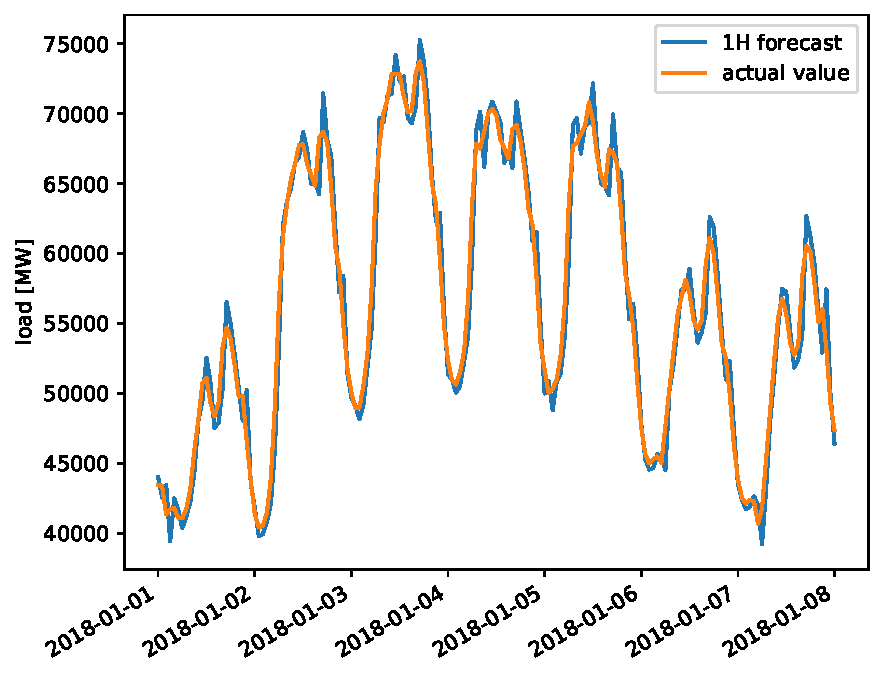
\includegraphics[width=\textwidth]{plots/ARMAXfc/ARMAX_p2q2_data2015to2017_fcto2018123100_plot_range2018010100_2018010800}%
\caption{An example forecast from 2017/12/31 01:00 to 2018/01/08 00:00 for an ARMAX(2,2) using load data from 2015/01/08 00:00 to 2017/12/31 00:00 for training.}%
\label{fig:armax_fc}%
\end{figure}

\begin{figure}[h!]%
\centering
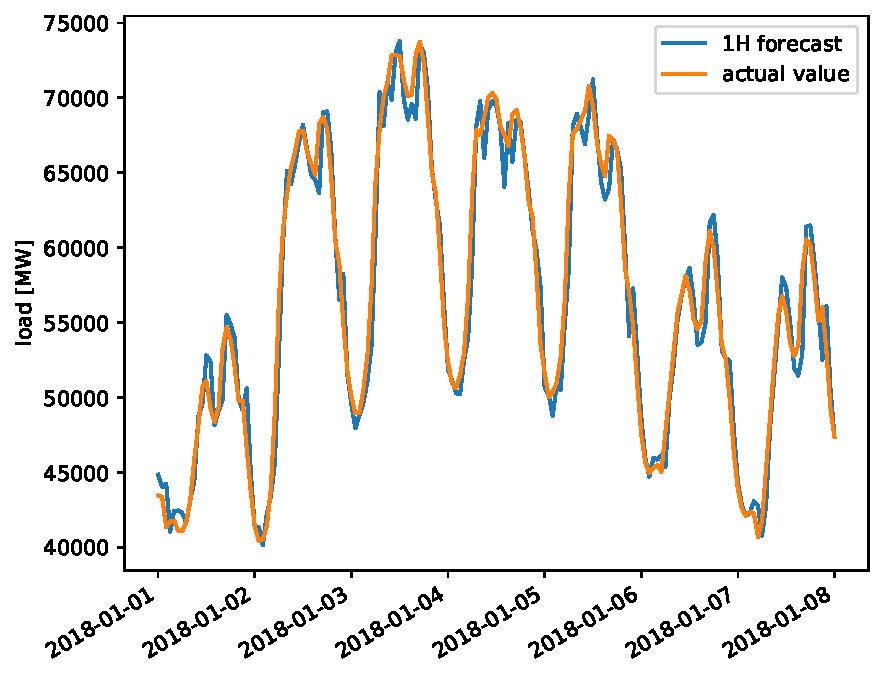
\includegraphics[width=\textwidth]{plots/ARMAXfc/ARMAX_p2q2_data2015to2017_fcto2018123100_t2m_top10_plot_range2018010100_2018010800}%
\caption{An example forecast from 2017/12/31 01:00 to 2018/01/08 00:00 for an ARMAX(2,2) using load data from 2015/01/08 00:00 to 2017/12/31 00:00 for training and the grid points of the ten regions with the highest population as exogenous input.}%
\label{fig:armax_fc_dayofweek}%
\end{figure}

\begin{figure}[h!]%
\centering
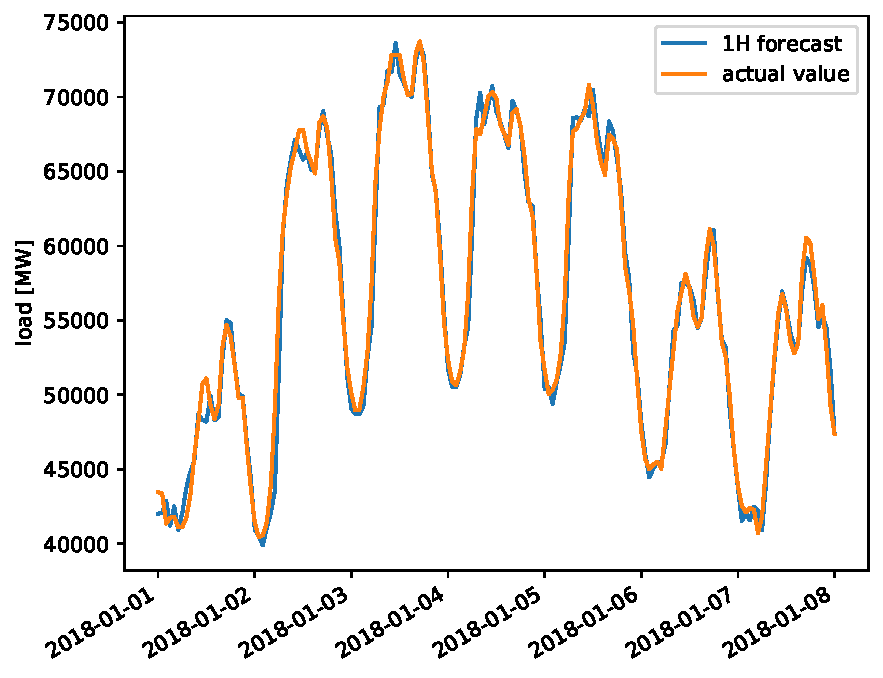
\includegraphics[width=\textwidth]{plots/ARMAXfc/ARMAX_p2q2_data2015to2017_fcto2018123100_load_lag_plot_range2018010100_2018010800}%
\caption{An example forecast from 2017/12/31 01:00 to 2018/01/08 00:00 for an ARMAX(2,2) using load data from 2015/01/08 00:00 to 2017/12/31 00:00 for training and the load data shifted back in time by one week for the same time range as exogenous input.}%
\label{fig:armax_fc_load_lag}%
\end{figure}%

\begin{figure}[h!]%
\centering
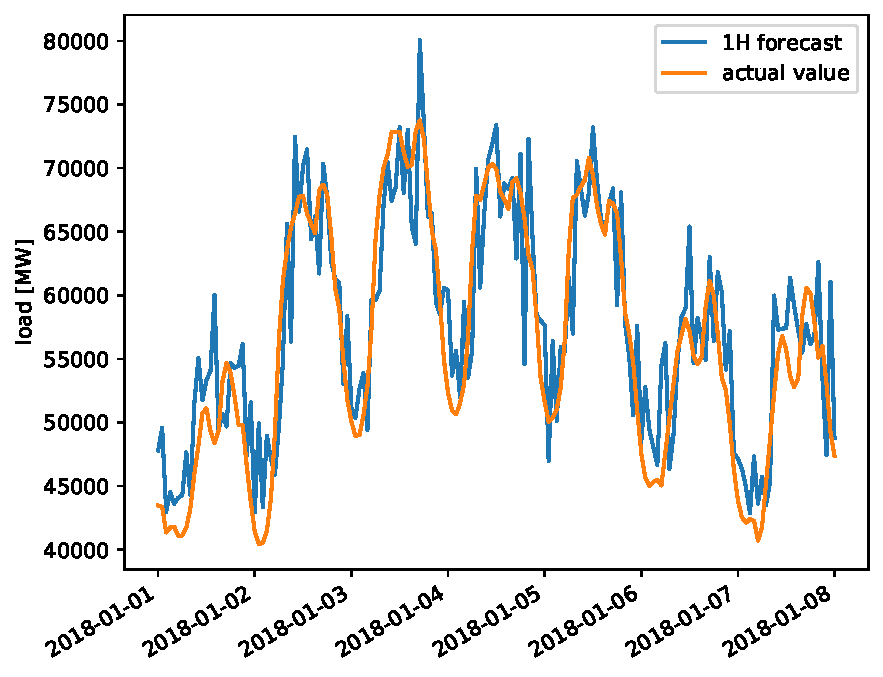
\includegraphics[width=\textwidth]{plots/ARMAXfc/ARMAX_p1q0_data2017010100to2017123100_fc2017123101to2018010800_t2m_all}%
\caption{An example forecast from 2017/12/31 01:00 to 2018/01/08 00:00 for an ARMAX(1,0) using load data from 2017/01/01 00:00 to 2017/12/31 00:00 for training and all 1435 grid points of the 2 metre temperature variable as exogenous inputs.}%
\label{fig:armax_fc_t2m_all}%
\end{figure}%



\begin{table}
\rowcolors{2}{white}{gray!25}
\centering
\caption{The names of the ten regions with the highest population and the actual population for 2018, respectively.}
\footnotesize
\begin{tabularx}{.6\linewidth}{p{6cm}r}
\tablehead region name & \tablehead population\\
Berlin & 3613495\\
Hamburg & 1830584\\
München, Kreisfreie Stadt & 1456039\\
Region Hannover & 1152675\\
Köln, Kreisfreie Stadt & 1080394\\
Frankfurt am Main, Kreisfreie Stadt & 746878\\
Stuttgart, Stadtkreis & 632743\\
Düsseldorf, Kreisfreie Stadt & 617280\\
Recklinghausen & 616824\\
Rhein-Sieg-Kreis & 599056\\
\end{tabularx}
\label{tab:top10_population}
\end{table}

In \Cref{tab:armax_forecast_table}, 168h shifted load means the time series, where the actual load data is shifted back in time by one week. The temp mean variable is the mean of the 2 metre temperature for each step in time, respectively. The data counter represents a counter, that counts the steps from 0 up to the length of the data. And last top 10 regions temp denotes the grid points of the 10 regions with the highest population, each grid point as a single time series.\\

As already can be estimated from the information criteria in \Cref{tab:ic_table}, there is a huge difference between the ARMA(1,0) and the ARMA(2,2) model. This results in a difference of more than 1.3\% of the \gls{mape} and can be observed in \Cref{tab:armax_forecast_table}. It can be seen, that of all exogenous variables used, including load data shifted by one week, has the greatest impact on the forecast error, causing these model to have the lowest error. In contrast to that, including the 10 regions with the highest population lead to a higher error. This could result from the high correlation between neighbouring grid points in single regions. The respective regions with the highest population are listed in \Cref{tab:top10_population}. A model for the 2 metre temperature with all grid points has been fitted too, but the number of 1435 exogenous variables implies a massive amount of computation time which is unpracticable for real-time forecasting. Furthermore, due to the high correlation between the different grid points, there is a high chance for errors during training. Also, a model with that many variables is prone to over-fitting and thus has a higher error on new data which can be seen in \Cref{fig:armax_fc_t2m_all}. It is very interesting that including the mean temperature seems to result in a slightly better result than using any constellation of single grid points such as \eg the 10 regions with the highest population.\\

\begin{sidewaystable}[!ht]%
\rowcolors{2}{white}{gray!25}
\centering
\caption{\acrshort{arma}/\acrshort{armax} performance using different input data. For each error metric, the field with the best value is highlighted in green.}
\footnotesize
\begin{tabularx}{\linewidth}{Xlllllrrrr}
\tablehead model & \tablehead 168h shifted load & \tablehead temp mean & \tablehead data counter & \tablehead weekend & \tablehead top 10 regions temp & \tablehead\gls{rmse} & \tablehead\gls{mae} & \tablehead\gls{mpe} & \tablehead\gls{mape}\\\hline
ARMA(1,0) & \xmark & \xmark & \xmark & \xmark & \xmark & 2621.940 & 1961.213 & 0.006 & 3.460\\
ARMA(2,2) & \xmark & \xmark & \xmark & \xmark & \xmark & 1727.742 & 1216.559 & 0.220 & 2.114\\
ARMAX(2,2) & \cmark & \cmark & \xmark & \xmark & \xmark & 1024.265 & 628.298 & -0.020 & \cellcolor{green!35}1.103\\
ARMAX(2,2) & \cmark & \cmark & \cmark & \xmark & \xmark & 1024.310 & 628.331 & -0.006 & \cellcolor{green!35}1.103\\
ARMAX(2,2) & \cmark & \cmark & \xmark & \cmark & \xmark & \cellcolor{green!35}1024.251 & \cellcolor{green!35}628.292 & -0.020 & \cellcolor{green!35}1.103\\
ARMAX(2,2) & \cmark & \cmark & \cmark & \cmark & \xmark & 1024.295 & 628.324 & -0.006 & \cellcolor{green!35}1.103\\
ARMAX(2,2) & \cmark & \xmark & \xmark & \xmark & \xmark & 1030.753 & 633.436 & 0.101 & 1.112\\
ARMAX(2,2) & \cmark & \xmark & \xmark & \cmark & \xmark & 1030.756 & 633.433 & 0.101 & 1.112\\
ARMAX(2,2) & \cmark & \xmark & \cmark & \xmark & \xmark & 1029.191 & 633.093 & -0.165 & 1.114\\
ARMAX(2,2) & \cmark & \xmark & \cmark & \cmark & \xmark & 1029.199 & 633.103 & -0.165 & 1.114\\
ARMAX(2,2) & \cmark & \xmark & \xmark & \xmark & \cmark & 1043.292 & 649.564 & -0.018 & 1.144\\
ARMAX(2,2) & \cmark & \xmark & \cmark & \xmark & \cmark & 1043.711 & 650.046 & -0.012 & 1.145\\
ARMAX(2,2) & \cmark & \xmark & \cmark & \cmark & \cmark & 1051.469 & 659.243 & -0.012 & 1.164\\
ARMAX(2,2) & \cmark & \cmark & \xmark & \cmark & \cmark & 1051.801 & 659.805 & -0.021 & 1.165\\
ARMAX(2,2) & \cmark & \cmark & \cmark & \cmark & \cmark & 1051.956 & 660.006 & \cellcolor{green!35}-0.004 & 1.165\\
ARMAX(2,2) & \cmark & \cmark & \xmark & \xmark & \cmark & 1062.208 & 667.663 & -0.011 & 1.179\\
ARMAX(2,2) & \cmark & \xmark & \cmark & \xmark & \xmark & 1656.760 & 1178.435 & 0.021 & 2.043\\
ARMAX(2,2) & \xmark & \cmark & \xmark & \xmark & \xmark & 1662.298 & 1179.187 & 0.185 & 2.039\\
ARMAX(2,2) & \xmark & \cmark & \xmark & \cmark & \xmark & 1661.909 & 1179.681 & 0.187 & 2.040\\
ARMAX(2,2) & \xmark & \cmark & \cmark & \cmark & \xmark & 1656.224 & 1179.021 & 0.022 & 2.044\\
ARMAX(2,2) & \xmark & \xmark & \cmark & \xmark & \xmark & 1730.620 & 1226.238 & -0.382 & 2.119\\
ARMAX(2,2) & \xmark & \xmark & \cmark & \cmark & \xmark & 1730.620 & 1226.237 & -0.382 & 2.119\\
ARMAX(2,2) & \xmark & \cmark & \cmark & \cmark & \cmark & 1811.407 & 1321.255 & 0.043 & 2.315\\
ARMAX(2,2) & \xmark & \xmark & \cmark & \xmark & \cmark & 2004.932 & 1444.396 & -0.036 & 2.547\\
ARMAX(2,2) & \xmark & \cmark & \cmark & \xmark & \cmark & 2032.248 & 1456.478 & -0.025 & 2.570\\
ARMAX(2,2) & \xmark & \xmark & \xmark & \xmark & \cmark & 2130.514 & 1508.978 & 0.211 & 2.663\\
%ARMAX(2,2) & \xmark & \xmark & \xmark & \xmark & \xmark & & & & \\
\end{tabularx}
\label{tab:armax_forecast_table}
\end{sidewaystable}

\newpage

%Describe the results you have obtained using your methods described above. Again use proper visualization methods.
